% !TEX root = ../YourName-Dissertation.tex

\chapter{Precise Analysis on Single-trace Attacks}\label{chapter4}

\section{Problem}
In Chapter~\ref{chapter3}, we present a method to identify address-based side-channel leakage sites in cryptography libraries ~\cite{Osvik2006,Gullasch:2011:CGB:2006077.2006784,203878,10.1007/978-3-540-45238-6_6}. However, many reported leakage sites are not patched by the developers. Recent work on side-channel vulnerability identification~\cite{203878,217537,Wichelmann:2018:MFF:3274694.3274741,Brotzman19Casym,236338,182946} also faced the same situation. For example, DATA~\cite{217537} reports 2,248 potential leakage sites for the RSA implementation in OpenSSL 1.1.0f\@. Further analysis shows 1,510 leaks can be dismissed, but that still leaves 460 data-access leaks and 278 control-flow leaks. Many of these vulnerabilities have not been fixed by the developers for a variety of reasons.

First, some vulnerable implementations perform better. For example,
RSA implementations usually adopt the Chinese Remainder Theorem (CRT) optimization, which is faster but vulnerable to fault attacks~\cite{aumuller2002fault}. Second, fixing old vulnerabilities can introduce new
weaknesses. Third, most vulnerabilities pose a negligible risk. Although some vulnerabilities result in the key being entirely compromised~\cite{184415, aumuller2002fault}, many others are less severe in reality. Therefore, we need a proper quantification metric to assess the sensitivity of side-channel vulnerabilities, so a developer can efficiently triage them.

Previous work on side-channel quantification~\cite{182946,5207642} can identify numerous leakages or even provide an upper bound on the amount of leakage, which is useful to verify that an implementation is secure if it incurs zero leakage.
However, these techniques cannot quantify the severity of a leak because they over approximate the leakage. For example, CacheAudit~\cite{182946}
reports that the upper-bound leakage of AES-128 exceeds the original key size. Besides, existing side-channel quantification work~\cite{182946,5207642} assumes an attacker runs the target program multiple times with different
input secrets and calculates an ``average'' estimation, which is different from real attack scenarios when the secret that an attacker wants to retrieve is fixed. As a consequence, these results are less useful in assessing the severity level of each leakage site.

To overcome these limitations, we propose a novel method to quantify information
leakage precisely. We quantify the number of bits that can be leaked during a real
execution and define the amount of leaked information as the cardinality of
possible secrets based on an attacker's observation. Before an attack, an adversary has a large but finite input space.
Whenever the adversary observes a leakage site, he can eliminate some impossible
inputs and reduce the input space's size. In an extreme case, if the input space's size reduces to one, an adversary has determined the input, which means all secret information (e.g., the entire secret key) is
leaked. By counting the number of inputs~\cite{10.1007/11499107_24}, we can quantify the information leakage precisely.
We use symbolic execution to generate constraints to model the relation
between the original sensitive input and an attacker's observations.
Symbolic execution provides fine-grained information, but it is expensive
to compute. Therefore, prior symbolic
execution work~\cite{203878,236338,Brotzman19Casym} either analyzes only
small programs or applies domain knowledge~\cite{203878} to simplify the analysis. We
examine the bottleneck of the trace-oriented symbolic execution and optimize it
to work for real-world crypto-systems.

We have implemented the proposed technique in a tool called \tool{} and demonstrated
it on real-world crypto libraries, including OpenSSL,
mbedTLS, Libgcrypt, and Monocypher.
We collect execution traces of these libraries and apply
symbolic execution to each instruction. We model
each side-channel leak as a logic formula. These
formulas precisely model side-channel vulnerabilities.
Then we use the conjunction of these formulas to model the
leaks at a statement that appears in different location in
the execution trace file (e.g., leaks inside a loop).
Finally, we introduce a Monte Carlo sampling method to estimate
the information leakage.
The experimental results confirm
that \tool{} precisely identifies previously known vulnerabilities and
reports how much information is leaked and which byte in the original sensitive
buffer is leaked. We also test \tool{} on side-channel-free algorithms.
\tool{} produces no false positives.
The result also shows the newer version of crypto libraries leak less information
than earlier versions.
\tool{} also discovers new vulnerabilities. With the help of \tool{},
we confirm that some of these vulnerabilities are severe.


%Based on the fixed attack target, we classify the software-based side-channel
%vulnerabilities into two categories: 1.\textit{secret-dependent control-flow
%transfers} and 2.\textit{secret-dependent data accesses} and model them with
%math formulas which constrain the value of sensitive information. We quantify
%the amount of leaked information as the number of possible solutions that are
%reduced after applying each constrains.


%Our method can identify and quantify address-based sensitive information
%leakage sites in real-world applications automatically. Adversaries can exploit
%different control-flow transfers and data-access patterns when the program
%processes different sensitive data. We refer them as the potential information
%leakage sites. Our tool can discover and estimate those potential information
%leakage sites as well as how many bits they can leak. We are also able to
%report precisely how many bits can be leaked in total if an attacker observes
%more than one site. We run symbolic execution on execution traces. We model
%each side-channel leakage as a math formula. The sensitive input is divided
%into several independent bytes and each byte is regarded as a unique symbol.
%Those formulas can precisely model every the side-channel vulnerability. In
%other words, if the application has a different sensitive input but still
%satisfies the formula, the code can still leak the same information.  
%Those information leakage sites may spread in the whole program and their
%leakages may not be dependent. Simply adding them up can only get a coarse
%upper bound estimate. In order to accurately calculate the total information
%leakage, we must know the dependent relationships among those multiple leakages
%sites. Therefore, we introduce a monte carlo sampling method to estimate the
%total information leakage.

In summary, we make the following contributions:

\begin{itemize}
    \item We propose a novel method that can quantify fine-grained leaked
          information from side-channel vulnerabilities that result from actual attack
          scenarios. Our approach differs from previous ones in that we
          model real attack scenarios for one execution.
          We model the information quantification problem as a counting problem
          and use a Monte Carlo sampling method to estimate the information leakage.

    \item We implement the method into a tool and apply it
          to several pieces of real software. \tool{} successfully identifies
          previous unknown and known side-channel vulnerabilities and calculates the corresponding information leakage.
          Our results are useful in practice.
          The leakage estimates and the corresponding trigger inputs can
          help developers to triage and fix the vulnerabilities.
\end{itemize}

\section{Threat Model}

The threat model in this chapter is similar to the threat model in our previous work from Chapter~\ref{chapter3}. Prior work~\cite{203878,182946,Brotzman19Casym} also shares the same threat model. That is, we assume
an attacker can share some hardware resource with the victim. The attacker has
the ability to probe the victim at any time of the execution. We also assume
an attacker has noise-free observations. The attacker has the access to the victim's
binary executable.  We believe that the majority of address-based side-channel attacks in the literature applies to the thread model.


\section{Background}
Given an event $e$ that occurs with the probability $p(e)$, we receive
\begin{displaymath}
    I = - \log_2p(e)
\end{displaymath}
bits of information by knowing the event $e$ happens according to information theory~\cite{shannon1948mathematical}.
Considering a char variable $a$
with one byte storage size in a C program, its value ranges from 0 to 255.
Assume $a$ has a uniform distribution. If we observe that
$a$ equals $1$, the probability of this observation is $\frac{1}{256}$. So
we get $-\log(\frac{1}{256}) = 8$ bits information, which is exactly the size
of a char variable in the C program.

Existing work on information leakage quantification typically uses Shannon
entropy~\cite{clark2007static,Wichelmann:2018:MFF:3274694.3274741},
min-entropy~\cite{10.1007/978-3-642-00596-1_21}, and max-entropy~\cite{182946,
    Doychev:2017:RAS:3062341.3062388}. In these frameworks, the input sensitive
information $K$ is considered as a random variable.

Let $k$ be one of the possible
value of $K$. The Shannon entropy $H(K)$ is defined as
\begin{displaymath}
    H(K) = - \sum_{k {\in} K}p(k)\log_2(p(k)).
\end{displaymath}

Shannon entropy can be used to quantify the initial uncertainty about the
sensitive information. It measures the amount of information in a system.

Min-entropy describes the information leaks for a program with the most likely input.
For example, min-entropy can be used to describe the
best chance of success in guessing one's password using the
most common password. %, which is defined as
\begin{displaymath}
    \mathit{min\text{-}entropy} = - \log_2(p_{\mathit{max}})
\end{displaymath}

Max-entropy is defined solely on the number of possible observations.
%It is equal to $-\log_2{n}$.
\begin{displaymath}
    \mathit{max\text{-}entropy} = -\log_2{n}
\end{displaymath}
As it is easy to compute, most recent works~\cite{182946,Doychev:2017:RAS:3062341.3062388} use max-entropy as the definition of
the amount of leaked information.

To illustrate how these definitions work, we consider the code
fragment in Figure~\ref{fig:side-channel}. It has two secret-dependent
control-flows, A and B.

\begin{figure}[h!]
    \centering
    \begin{lstlisting}[xleftmargin=.1\textwidth, xrightmargin=.1\textwidth]
uint8_t key[2], t1, t2;
get_key(key);              // 0 <= key[0], key[1] < 256
t1 = key[0] + key[1];
t2 = key[0] - key[1];
if (t1 < 4){               // leakage site A
    foo();    
}                          
if (t2 > 0){               // leakage site B     
    doo();    
}                          
\end{lstlisting}
    \caption{Side-channel leakage}
    \label{fig:side-channel}
\end{figure}
In this chapter, we assume an attacker can observe the secret-dependent control-flows in Figure~\ref{fig:side-channel}.
Therefore, an attacker can have two different observations for each leak site
depending on the value of the $\mathit{key}$: $A$ for function \textsf{foo} is executed,
$\neg A$ for function \textsf{foo} is not executed, $B$ for function \textsf{doo} is
executed, and $\neg B$ for function \textsf{doo} is not executed. Now the
question is how much information can be leaked from the above code if an
attacker knows which branch is executed?

\begin{table}[ht]
    \centering%\small\footnotesize
    \caption{The distribution of observations}\label{shtable}
    %    \resizebox{\columnwidth}{!}{
    \begin{tabular}{l|cc|cc}
        \hline

        Observation ($o$)   & $A$    & $\neg A$ & $B$   & $\neg B$ \\ \hline
        Number of Solutions & 65526  & 10       & 32768 & 32768    \\ \hline
        Possibility (p)     & 0.9998 & 0.0002   & 0.5   & 0.5      \\
        \hline
    \end{tabular}
    %        }
\end{table}

Assuming $\mathit{key}$ is uniformly distributed, we can calculate the corresponding
possibility by counting the number of possible inputs. Table~\ref{shtable}
describes the probability of each observation. We use the above three types of
leakage metrics to calculate the amount of leaked information for leak A and leak B.

\subsubsection*{Min Entropy}
As $p_{A\mathit{max}} = 0.9998$ and $p_{B\mathit{max}} = 0.5$,
with the definition, min-entropy equals to
\begin{align*}
    \mathit{min\text{-}entropy_A} & = -\log_2{0.9998} = 0.000\ \mathrm{bits} \\
    \mathit{min\text{-}entropy_B} & = -\log_2{0.5} = 1.000\ \mathrm{bits}
\end{align*}

\subsubsection*{Max Entropy}
Depending on the value of key, the code can run two different branches for each leakage site.
Therefore, with the max entropy
definition, both leakage sites leak

\begin{displaymath}
    \mathit{max\text{-}entropy} = -\log_2{2} = 1.000\ \mathrm{bits}
\end{displaymath}

\subsubsection*{Shannon Entropy}
Based on Shannon entropy, the respective amount of information in A and B equals to
    {%\footnotesize
        \begin{align*}
            \mathit{Shannon\text{-}entropy_A} & = -(0.9998*\log_{2}0.9998      \\
                                              & \qquad+ 0.0002*\log_{2}0.0002) \\
                                              & = 0.000\ \mathrm{bits}         \\
            \mathit{Shannon\text{-}entropy_B} & = -(0.5*\log_{2}0.5 + 0.5*\log_{2}0.5)       \\
                                              & = 1.000\ \mathrm{bits}
        \end{align*}
    }
In the next section, we will show that these measures work well only
theoretically in a static analysis setting.
Generally, they do not apply to dynamic analysis or real
settings. We will present that the static or theoretical results could be
dramatically different from the real world, and we do need a better method to
quantify the information leakage from a practical point of view.

\section{Leakage Definition}

In this section, we discuss how \tool{} quantifies the amount of leaked
information. We first present the limitation of existing quantification metrics.
Then, we introduce our model, the mathematical notation used in the
chapter, and our method.

\subsection{Problem Setting}
Existing static side-channel quantification
works~\cite{182946,Wichelmann:2018:MFF:3274694.3274741,zhang2010sidebuster,bang2016string} define information
leakage using max entropy or Shannon entropy.  If zero bits of
information leakage is reported, a program is secure. However, when a tool using these metrics reports leakage, it is the ``average'' leakage. In a real attack, the leakage could be dramatically different.

\begin{figure}[h!]
    \centering
    \begin{lstlisting}[xleftmargin=.1\textwidth, xrightmargin=.1\textwidth]
char key[9] = input();
if(strcmp(key, "password"))   // leakage site C
    pass();                   // branch 1
else
    fail();                   // branch 2
\end{lstlisting}
    \caption{A dummy password checker}
    \label{fig:password-checker}
\end{figure}

Consider a password checker sketched in Figure~\ref{fig:password-checker}.
The password checker takes an 8-byte char array (exclude \textsf{NULL} character)
and checks if the input is the correct password. If an attacker uses a side-channel attack to determine that the code executes branch
$\{{1\}}$, they can infer that the password equals to
``password'', in which case the attacker retrieves the full password.
Therefore, the total leaked information should be 64 bits, which equals to the
size of the original sensitive input when the code executes branch
$1$.

However, prior static approaches cannot precisely capture the amount of leakage. According to the definition of Shannon entropy, the leakage will be
$$\frac{1}{2^{64}}*\log_{2}\frac{1}{2^{64}} + \frac{2^{64}-1}{2^{64}}
    *\log_{2}\frac{2^{64}-1}{2^{64}} \approx 0\, \mathrm{bits}.$$ Max-entropy is defined from the
number of possible observations. Because the program has two
branches, tools based on max-entropy will report the code has a $\log_2{2} = 1.0$
bit leakage.
Both approaches fail to tell how much information is leaked during the execution
precisely. The problem with existing methods is that they are static-based so
input values and real runtime information are neglected by their approaches.
They assume an attacker runs
the program multiple times with many different or random sensitive inputs. As
shown in Figure~\ref{fig:gap}(a), previous methods, both Shannon entropy and max
entropy, give an ``average'' estimate of the information leakage. However, it is
not the typical scenario for an adversary to launch a side-channel attack. When
a side-channel attack happens, the adversary wants to retrieve the sensitive
information, in which case the sensitive information is fixed (e.g., AES keys).
The adversary will run the attack over and over again with fixed input and
guess the value bit by
bit (e.g., Kocher's timing attacks~\cite{kocher1996timing}), as in Figure~\ref{fig:gap}(b). We want to have a
theory for dynamic analysis that if the theory says an attack leaks $x$ bits of
secret information from a side-channel vulnerability, then $x$ should be useful
in estimating the sensitive level of the vulnerability. However, the above
methods all fail in real attack models.
\begin{figure}
    \centering
    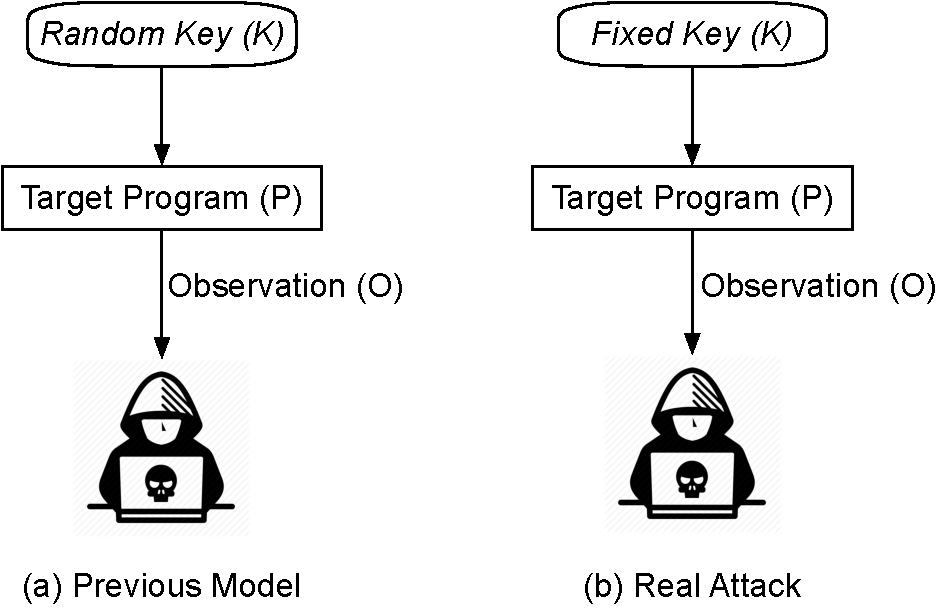
\includegraphics[width=.65\columnwidth]{./figures/chapter4/RA.pdf}
    \caption{The gap between real attacks and previous models}\label{fig:gap}
\end{figure}

\subsection{Precise Analysis}
Now we present our metric to quantify the amount of leaked information from
dynamic analysis.

We assume a program ($\beta$) has $K$ as its sensitive input. The input $K$ should be
a finite set of keys. The program also takes known messages $M$ as its input.
During an AES encryption, for example,
$\beta$ is the encryption function. Here $K$ is the set of all possible AES keys,
and $M$ represents the set consisting of all plaintext messages to be encrypted. In a real execution, an adversary may have
some observations ($O$) of the program. This dissertation only
uses secret-dependent control flows and secret-dependent data
accesses as observations.

With the above definition, we have the following mapping between $\beta$,
$K$, $M$, and $O$:

\begin{displaymath}
    \beta(K, M) \rightarrow O.
\end{displaymath}


We model a side-channel in the following way. An adversary does not have
access to $K$, but he knows $\beta$, $M$, and $O$. For one execution of a
deterministic program, once $k \in K$ and $m \in M$ are fixed, the observation
($o \in O$) should also be determined. An attacker knows $\beta$, $o$,
and $m$. The attacker wants to infer the value of $k$. We use $K^o$ to denote
the set of possible $k$ values that produce the same observation: $K^o = \{ k \in K \, |\, \beta(k, m) \rightarrow o\}$

Then the problem of quantifying the amount of leaked information can be
restated as the following question:

\
\emph{How much uncertainty of $K$ is reduced if an attacker knows $\beta$, $m$, and $o$?}
\

In information theory, the mutual information ($I$) is a measure of the mutual
dependence between two variables. Here we use $I$ to describe the
dependence between original sensitive keys ($K$) and attackers' observations ($O$),
which is defined as

\begin{equation} \label{eq:1}
    I(K;O) = \sum_{k {\in} K}{\sum_{o {\in} O}{p(k, o)\log_2\frac{p(k, o)}{p(k)p(o)}}},
\end{equation}

\noindent where $p(k_i, o_i)$ is the joint discrete distribution of $K$ and $O$.
Alternatively, the mutual information can also be equivalently expressed as

\begin{equation} \label{eq:2}
    I(K;O) = H(K) - H(K|O),
\end{equation}

\noindent where $H(K|O)$ is the entropy of $K$ with the condition $O$. It quantifies the
uncertainty of $K$ given the value of $O$. In other word, the conditional
entropy $H(K|O)$ marks the uncertainty about $K$ after an adversary has gained
some observations ($O$).
\begin{equation}
    H(K|O) = - \sum_{o {\in} O} {p(o) \sum_{k {\in} K}{p(k|o)\log_2p(k|o)}}
\end{equation}

In this research, we hope to give a very precise definition of information
leakages. Suppose an attacker runs the target program with one
fixed input, we want to know how much information he can infer by observing the
memory access patterns ($o$). We come to the simple slogan
~\cite{10.1007/978-3-642-00596-1_21} %% where the information
%% leakage equals:
%% \textbf{Initial uncertainty - remaining uncertainty}
that
\begin{align*}
     & \mathit{Information\ leakage} =                                       \\
     & ~~~~ \mathit{Initial\ uncertainty} - \mathit{Remaining\ uncertainty}.
\end{align*}

Next we compare the Eq.~(\ref{eq:2}) with the above slogan, we find that $H(K)$
is the $\mathit{Initial\ uncertainty}$ and $H(K|O)$ is the $\mathit{Remaining\
        uncertainty}$. During a real attack, the observation ($o$) is known.  Thus we
have $H(K|O) = H(K|o)$.

Therefore, we define the amount of leaked information as
\begin{displaymath}
    Leakage = I(K;o) = H(K) - H(K|o).
\end{displaymath}

For a program ($\beta$) without knowing any domain information, all possible sensitive
inputs should appear equally. Therefore, for any $k \in K$, $p(k) =
    \frac{1}{|K|}$. So we have
$$H(K) = \sum_{k {\in} K}\frac{1}{|K|}\log_2{|K|} = \log_2{|K|}.$$
For any $k' \in K \setminus K^o$, $p(k'|o) = 0$. We get
\begin{align*}
    I(K;o) & = - \sum_{k {\in} K^o}{p(k|o)\log_2p(k|o)}                         \\
           & \qquad   - \sum_{k` {\in} (K \setminus K^o)}{p(k'|o)\log_2p(k'|o)} \\
           & = \sum_{k {\in} K^o}\frac{1}{|K^o|}\log_2{|K^o|}                   \\
           & = \log_2{|K^o|}.
\end{align*}


\begin{mydef}
    \label{chapter4:def}
    Given a program $\beta$ with the input set $K$,
    an adversary has the observation $o$ when the input $k{\in}K^o$.
    We denote it as
    $$\beta(K^o, m) \rightarrow	o.$$

    The amount of leaked information $L_{\beta(k)\rightarrow o}$ based on the observation ($o$) is
    $$L_{\beta(k)\rightarrow o} = \log_2{|K|} - \log_2{|K^o|}.$$
\end{mydef}

The above definition~\cite{AskarovC12} can be understood in an intuitive way. Suppose an attacker
wants to guess a 128-bit encryption key from a program.
Without any domain knowledge,
he can find the key by performing exhaustive search over $2^{128}$ possible keys.
However, the program has a side-channel leakage site. After the program finishes execution, the
attacker gets some leaked information and only needs to find the key by performing
exhaustive search over $2^{120}$ possible keys. Then we can say that 8 bits of the information
is leaked. In this example, $2^{128}$ is the size of $K$ and $2^{120}$ is the size of $K^o$.


With the definition, if an attacker observes that the code in
Figure~\ref{fig:password-checker} runs the branch 1, then the $K^{o^{1}} =
    \{\mathrm{``password"}\}$. Therefore, the information leakage $L_{P(k)=o^{1}} =
    \log_2{2^{64}} - \log_2{1} = 64$ bits, which means the key is totally leaked. If
the attacker observes the code hits branch 2, the leaked information is
$L_{P(k)=o^{2}} = \log_2{2^{64}} - \log_2{(2^{64}-1)} \approx 0$ bit.


We can also calculate the leaked information from the sample code in
Figure~\ref{fig:side-channel}. As the size of input sensitive information is
usually public. The problem of quantifying the leaked information has been
transferred into the problem of estimating the size of input key $|K^o|$ under
the condition $o \in O$. The result is shown in Table~\ref{shtable2}. We can see
that some branches (e.g., A) or traces leak much more information than some others.
These kinds of branches can be vulnerable when an attacker's data is incorporated.
For example, the code will skip some of the calculation if the value is 0 in big
number multiplication.

In contrast, an \emph{average} estimate based on random secret input information is around $1$ bit, as shown in the previous section and Table~\ref{shtable}, is not very useful in practice as an attacker is able to get much more leaked
information in some attack scenarios. As the size of input-sensitive information is
usually public, the problem of quantifying the leaked information is equivalent to the problem of estimating the size of input key $|K^o|$ under
the condition $o \in O$. 

\begin{table}[ht]
    \centering%\small\footnotesize
    \caption{New leakage modeling results}
    \label{shtable2}
    %    \resizebox{\columnwidth}{!}{
    \begin{tabular}{l|cc|cc}
        \hline

        Observation ($o$)         & $A$   & $\neg A$ & $B$   & $\neg B$ \\ \hline
        Number of Solutions       & 65526 & 10       & 32768 & 32768    \\ \hline
        Leaked Information (bits) & 0.0   & 14.7     & 1.0   & 1.0      \\
        \hline
    \end{tabular}
\end{table}

\section{Approximate Model Counting}
\label{MCreasons}
In the previous section, we propose an information leakage definition for realistic attack scenarios to model two types of address-based side-channel leakages and show how to quantify them by calculating the number of input keys ($K^o$) that satisfy the formulas. Intuitively, we can use symbolic execution to capture math formulas and model counting to obtain the number of satisfying input keys ($K^o$). However, some preliminary experiments showed that this approach was far too expensive to use with real-world applications. In this section, we discuss the bottlenecks in this approach and propose a practical solution.


According to Definition~\ref{chapter4:def} introduced in the previous section,
the problem of quantifying the amount of leaked information can be reduced to
the problem of computing the number of items in $K^o$. However, we find that while
there are various propositional model counters (e.g., \#SAT), they are not
sufficiently scalable for production cryptosystem analysis.
Besides, there is no open source modulo theories counter (\#SMT) available.

One straightforward method to approximate the number of solutions is based on Monte Carlo
sampling. However, the number of satisfying values could be exponentially small.
Consider the formula $f_i\equiv{k_1} = 1\land{k_2} = 2\land{k_3} = 3\land{k_4} =
    4$, where $k_1$, $k_2$, $k_3$, and $k_4$ each represents one byte in the
original sensitive input buffer, there is only one satisfying solution of total
$2^{32}$ possible values, which requires exponentially many samples to get a
tight bound. Monte Carlo method also suffers from the curse of dimensionality.
For example, the length of an RSA private key can be as long as 4096 bits. If we
take each byte (8 bits) in the original buffer as one symbol, the formula can
have as many as 512 symbols.

We adopt multiple-step Monte Carlo sampling methods to count the number of
possible inputs that satisfy the logic formula groups. The key idea is to split
these constraints into several small formulas and sample them independently.
We will introduce the method in the following subsection. In this section, we present the algorithm to calculate the information leakage based on Definition~\ref{chapter4:def}. 


\newcommand{\addr}[1]{{l}_{#1}}
\renewcommand{\addr}[1]{{\gamma}_{#1}}
\renewcommand{\addr}[1]{{\zeta}_{#1}}
\renewcommand{\addr}[1]{{\xi}_{#1}}



\subsection{Problem Statement}
For each leakage site, we model it with a constraint using the
method presented in the previous section. Suppose the address of the leakage site is $\addr{i}$, we use $c_{\addr{i}}$ to denote the constraint that models its side-channel leakage. For multiple leakage sites, we take the conjunction of these constraints to represent these leakage sites.

According to Definition~\ref{chapter4:def}, to calculate the amount of leaked
information, the key is to calculate the cardinality
of $K^o$. Suppose an attacker can observe $n$ leakage sites, and each leakage
site has the following constraints: $c_{\addr{1}}, c_{\addr{2}}, \ldots,
    c_{\addr{n}}$ respectively. The total leakage can be calculated from the constraint
$c_t({\addr{1}},{\addr{2}},\ldots,{\addr{n}}) = c_{\addr{1}} \land c_{\addr{2}}
    \land \ldots \land c_{\addr{n}}$.
The problem of estimating the total leaked
information can be reduced to the problem of counting the number of different
solutions that satisfies the constraint
$c_t({\addr{1}},{\addr{2}},\ldots,{\addr{n}})$.
A simple method is to pick elements $k$ from $K$ and check if an
element is also contained in $K^o$. Assume $q$ elements satisfy this condition. In
expectation, we can use $\frac{k}{q}$ to approximate the value of
$\frac{|K|}{|K^o|}$.

However, the above sampling method fails in practice due to the following two problems.

\begin{enumerate}
    \item The curse of dimensionality problem. $c_t({\addr{1}},\ldots,{\addr{n}})$ is
          the conjunction of many constraints. Therefore, the input variables
          of each constraints will also be the input variables of the
          $c_t({\addr{1}},\ldots,{\addr{n}})$. The sampling method fails
          as $n$ grows.
          For example, if the program has $2$ input whose size is
          one byte, the whole search space is a $256^2$ cube. If we want
          the sampling distance between each point equals to $d$, we need
          $256^2d$ points. If the program has $10$ byte input, we need
          $256^{10}d$ points if we still we want the sampling distance equals
          to $d$.

    \item The number of satisfying assignments could be exponentially small.
          According to the Chernoff bound~\cite{hoeffding1994probability}, we need exponentially many samples to
          get a tight bound.
          On an extreme situation, if the constraint only
          has one unique satisfying solution, the simple Monte Carlo method
          cannot find the satisfying assignment even after sampling many
          points.
\end{enumerate}

However, despite the above two problems, we also observe two characteristics of the
problem:
\begin{enumerate}
    \item $c_t({\addr{1}},{\addr{2}},\ldots,{\addr{n}})$ is the conjunction of
          several short constraints $c_{\addr{i}}$. The set containing the
          input variables of $c_{\addr{i}}$ is the subset of the input
          variables of $c_t({\addr{1}},{\addr{2}},\ldots,{\addr{n}})$. Some
          constraints have completely different input variables from other
          constraints.

    \item Each time when we sample $c_t({\addr{1}},{\addr{2}},\ldots,{\addr{n}})$
          with a point, the sampling result is \emph{Satisfied} or not \emph{Not Satisfied}.
          The outcome does not depend on the result of
          previous experiments. Also, as the amount of leaked information is calculated
          by a $\log$ function, we need not exactly count the number of solutions for
          a given constraint.


\end{enumerate}

In regard to the above problems, we present our methods. First, we split
$c_t(\addr{1},\addr{2},\ldots,\addr{n})$ into several independent constraint
groups. After that, we run a multi-step sampling method for each constraint.

\subsection{Maximum Independent Partition}

For a constraint $c_{\addr{i}}$, we define function $\pi$, which projects the
constraint into a set of different input symbols. For example, $\pi(k1 + k2 >
    128) = \{k1, k2\}$.

\begin{mydef}[]
    \label{independentC}
    Given two constraints $c_m$ and $c_n$, we call them independent iff
    $$\pi(c_m) \cap \pi(c_n) = \emptyset$$
\end{mydef}

Based on Definition~\ref{independentC}, we can split the constraint
$c_t(\addr{1},\addr{2},\addr{3},\ldots,\addr{n})$ into several independent constraints.
There are many partitions. For our project, we are interested in the following
one.

\begin{mydef}\label{Goodpartition}
    For the constraint $c_t(\addr{1},\addr{2},\ldots,\addr{n})$,
    we call the constraint group
    $g_{1}, g_{2}, \ldots, g_{m}$
    the maximum independent partition of $c_t(\addr{1},\addr{2},\ldots,\addr{n})$ iff
    \begin{enumerate}
        \item $g_{1} \land g_{2} \land \ldots \land g_{m} = c_t(\addr{1},\addr{2},\ldots,\addr{n})$
        \item $\forall i, j \in \{1, \ldots, m\} \quad \textrm{and} \quad
                  i \neq j,\quad\pi(g_{i}) \cap \pi(g_{j}) = \emptyset $
        \item For any other partitions  $h_{1}, h_{2}, \ldots, h_{m'}$ satisfy 1) and
              2), $m \geq m'$
    \end{enumerate}

\end{mydef}

The reason we want a good partition of constraints is we want to reduce
the dimensions. For example,
a good partition of $F: ({k_1} = 1)\land({k_2} = 2)\land({k_3} > 4)\land({k_3} - {k_4} > 10)$ would be
$g_{1}: ({k_1} = 1)\quad g_{2}: ({k_2} = 2)\quad g_{3}: ({k_3} > 4) \land
    ({k_3} - {k_4} > 10)$
We can sample each constraint independently and combine them
with Theorem~\ref{IndependentConstraint}.

\begin{theorem}
    \label{IndependentConstraint}
    Let $g_{1}, g_{2}, \ldots, g_{m}$ be a maximum independent partition of
    $c_t(\addr{1},\addr{2},\ldots,\addr{n})$.
    $K_c$ is the input set that satisfies constraint $c$. We have the following
    equation with regard to the size of $K_c$
    $$|K_{c_t(\addr{1},\addr{2},\ldots,\addr{n})}| = |K_{g_{1}}| \cdot |K_{g_{2}}| \cdot \ldots \cdot|K_{g_{n}}|$$
\end{theorem}
With Theorem~\ref{IndependentConstraint}, we change the problem of counting the number of solutions to a complicated constraint in a high-dimension
space into counting solutions to several small constraints. We compute the maximum independent partition by iterating each $\addr{i}$ and applying the function $\pi$ over the constraint $\addr{i}$.

We apply 
Algorithm~\ref{algo:max-inde} to get the Maximum Independent Partition of the
$c_t(\addr{1},\addr{2},\ldots,\addr{n})$.


\IncMargin{1em}
\begin{algorithm}[th]\normalsize
    \DontPrintSemicolon
    \SetKwInOut{Input}{input}\SetKwInOut{Output}{output}
    \Input{$c_t(\addr{1},\addr{2},\ldots,\addr{n}) = c_{\addr{1}} \land c_{\addr{2}} \land \ldots \land c_{\addr{m}}$}
    \Output{The Maximum Independent Partition of $G = \{g_{1}, g_{2}  , \ldots,  g_{m} \}$ }
    Insert $c_{\addr{1}}$ to $G$ as a new entry \;
    \For{$i\leftarrow 2$ \KwTo $n$}
    {
        $S_{c_{\addr{i}}}$ $\leftarrow$ $\pi(c_{\addr{i}})$ \;
        \For{$g_{i} \in G$}
        {
            $S_{g_j}$ $\leftarrow$ $\pi(g_{j})$ \;
            $S$ $\leftarrow$ $S_{c_{\addr{i}}} \cap S_{g_j}$  \;
            \If{$S \neq \emptyset$}
            {
                $g_{j} \leftarrow g_{i} \land g_{\addr{i}}$ \;
                \textbf{continue} \;
            }
            Insert $c_{\addr{i}}$ to $G$ as a new entry \;
        }
    }
    \caption{The Maximum Independent Partition}
    \label{algo:max-inde}
\end{algorithm}
\DecMargin{1em}


\subsection{Multiple-step Monte Carlo Sampling}

After we split these constraints into several small constraints, we count the number of solutions for each constraint. Even though the dimension has been
significantly reduced by the previous step, this is still a \#P problem. For our project, we apply the approximate counting instead of exact counting for two reasons. First, we do not need to have a very precise result of the exact number of total solutions since the information is defined with a logarithmic function. We do not need to distinguish between constraints having $10^{10}$ or $10^{10} + 10$ solutions; they are very close to after taking logarithmic. Second, the
precise model counting approaches, such as Davis-Putnam-Logemann-Loveland (DPLL)
search, have difficulty scaling up to large problem sizes.

We apply the ``counting by sampling'' method. For
the constraint $g_{i}= c_{i_1} \land c_{i_2} \land ,\ldots, \land c_{i_j}\\ \land ,\ldots, \land c_{i_m}$, if the solution satisfies $g_{i}$, it should also
satisfy any constraint from $c_{i_1}$ to $c_{i_m}$. In other words, $K_{c_gi}$
should be the subset of $K_{c_1}$, $K_{c_2}$, \ldots , $K_{c_m}$. We notice that
$c_i$ usually has fewer inputs than $g_{i}$. For example, if
$c_{i_j}$ has only one 8-bit input variable, we can find the exact solution set
$K_{c_{i_j}}$ of $c_{i_j}$ by trying every possible 256 solution. After that,
we only generate random input numbers for the other input variables in
constraint $g_{i}$. With this simple yet effective trick, we reduce the number of input while still ensuring accuracy. The details of the algorithm is shown in Algorithm~\ref{chapter4:alg2}.


\IncMargin{1em}
\begin{algorithm}\normalsize
    \SetAlgoLined
    \DontPrintSemicolon

    \KwIn{{The constraint $g_{i}= c_{i_1} \land c_{i_2}
                    \land \ldots \land c_{i_m}$}}
    \KwOut{{The number of assignments that satisfy $g_{i}$ $|K_{g_{i}}|$}}

    $n$: the number of sampling times \;
    $S_{c_i}$: the set contains input variables for $c_{i}$ \;
    $n_{s}$: the number of satisfying assignments \;
    $N_{c_t}$: the set contains all solution for $c_t$ \;
    $r$: times of reducing $g$\;
    $k$: the input variable \;
    $R$: a function that produces a random point from $S_{c_i}$\;
    %$\#k$: the satisfying number of k \fixme{this number is not used syntactically} \;
    %Initialization: \;
    $r$ $\leftarrow$ $1$,
    $n$ $\leftarrow$ $0$ \;
    \For{$t$ $\leftarrow$ $1$ \KwTo $m$} {
    $S_{c_t}$ $\leftarrow$ $\pi(c_t)$ \;
    \If{$|S_{c_t}| = 1$}
    {
    $N_{c_t}$ $\leftarrow$ Compute all solutions of $c_i$ \;
    $N_{c_t} = \{n_1, \ldots, n_m\},\ S_{c_t} = \{k\}  $ \;
    $g_{i} = $ $g_i(k=n_1) \land \ldots \land g_i(k=n_m)$ \;
    $r \leftarrow r+1$ \;

    }
    }
    \While{$n \leq \frac{8p}{1-p}$} {
        $S_{g_i}$ $\leftarrow$ $\pi(g_i)$ \;
        $v \leftarrow R(S_{g_i})$ \;
        \If{$v$ satisfies $g_i$}
        {
            $n_s \leftarrow n_s + 1$
        }
        $n \leftarrow n +1,\ p = \frac{n_s}{n}$
    }

    $|K_{g_{i}}|$ $\leftarrow$ $n_s|K| / (n * r * \mathrm{range(k)})$
    \caption{Multiple Step Monte Carlo Sampling}\label{chapter4:alg2}
\end{algorithm}
\DecMargin{1em}

\subsection{Error Estimation}
\label{sssec:errest}
Our result has a probabilistic guarantee that the error of the estimated amount of leaked
information is less than 1 bit under the Central Limit Theorem (CLT) and uncertainty
propagation theorem~\cite{walpole1993probability}.

Let $n$ be the number of samples and $n_s$ be the number of samples that satisfy
the constraint $C$. Then we get $\hat{p} = \frac{n_s}{n}$. If we repeat the
experiment multiple times, each time we get a $\hat{p}$. As each
$\hat{p}$ is independent and identically distributed, according to the central limit
theorem, the mean value should follow the normal distribution
$$ \frac{\bar{p}-E(p)}{\sigma\sqrt{n}} \rightarrow N(0,1). $$ Here $E(p)$ is the
mean value of $p$, and $\sigma$ is the standard variance of $p$. If we use the
observed value $\hat{p}$ to calculate the standard deviation, we can claim that
we have 95\%\footnote{For a normal distribution, 95\% of variable $\Delta p$ fall within two sigmas of the mean.}
confidence that the error $\Delta p= \bar{p} - E(p)$ falls in the interval:
$$ |\Delta p| \leq 1.96\sqrt{\frac{ \hat{p} (1- \hat{p} )}{n}}.$$

Since we use $L = \log_{2}p$ to estimate the amount of leaked information, we
can have the following error propagation formula $\Delta L = \frac{\Delta
        p}{p\ln2}$ by taking the derivative from Definition~\ref{chapter4:def}. For \tool, we want the error of estimated leaked
information ($\Delta L$) to be less than 1 bit. So we get $\frac{\Delta
        p}{p\ln2} \leq 1$. Therefore, as long as $$ n \geq \frac{1.96^2(1-p)}{p(\ln2)^2},$$ 
\noindent we have 95\% confidence that the error of estimated leaked information is less than 1 bit.
During the simulation, if $n$ and $p$ satisfy this inequality, the Monte Carlo
simulation will terminate.

\section{Design and Implementation}

Figure~\ref{fig:workflow} shows the three steps of \tool{}.
First, we run the target program with a
concrete input (sensitive information) under the dynamic binary instrumentation
(DBI) framework to collect an execution trace. After that, we run the symbolic
execution to capture fine-grained semantic information for each
secret-dependent control-flow transfer and data access. Finally, we run Monte
Carlo (MC) simulation to estimate the amount of leaked information.

\begin{figure}[ht]
    \centering
    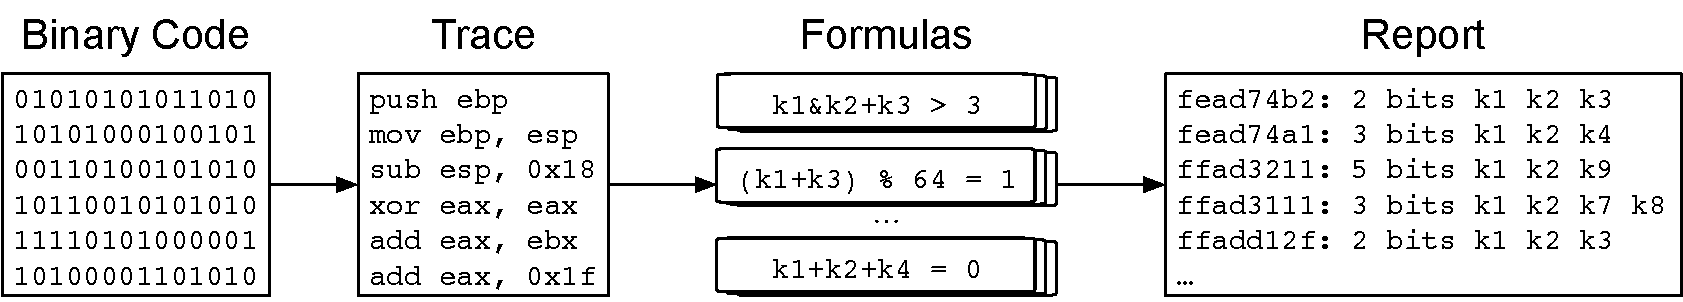
\includegraphics[width=0.95\textwidth]{./figures/chapter4/workflow.pdf}
    \caption{The workflow of \tool{}.}
    \label{fig:workflow}
\end{figure}

\subsection{Execution Trace Generation} The design goal of \tool{} is to estimate the information leakage as precisely as possible.
We run the target binary under a dynamic binary instrumentation (DBI) tool
to record execution traces and runtime information.
Once the sensitive information is loaded into memory, we start to collect the trace.
In this step, we mark variables and buffers that hold the sensitive data by either annotating the source code (\textsf{make\_abacus\_symbolic}) or telling the DBI tool of the memory address and the length of secrets.

\subsection{Instruction Level Symbolic Execution} We model an attacker's
observations from side-channel vulnerabilities with logic formulas.
Each formula captures the fine-grained information between the input
secrets and leakage sites. The engine only symbolically executes
instruction that might be affected by the input sensitive data. \tool{} works on one path at a time. The memory model is conceptually similar to other offline executors (e.g., SAGE~\cite{godefroid2008automated} and the trace-based executor of BitBlaze~\cite{song2008bitblaze}). That is, we use symbolic execution to track secrets. When secrets are loaded into the memory, \tool{} starts to interpret instructions symbolically. We treat secrets as symbols ($S$). For other variables, we use concrete values ($C$) from the execution. We do not know which instruction may manipulate a secret until we execute it. For each instruction, if all its operands and implicit memory accesses are concrete values, we perform concrete calculation and update the destination with the concrete value according to the instruction semantics. Otherwise, we symbolically interpret the instruction and update the destination with a formula.

\subsection{Leakage Estimation} 
We change the information leakage quantification problem into the counting problem. We propose a
Monte Carlo method to estimate the number of satisfying solutions. With the help of the Central Limit Theorem (CLT), we also give an error
estimate with the probability, which provides us with the \emph{precision guarantee}.

\subsection{Implementation}

\tool{} consists of 16,729 lines of code in C++17 and Python. It has three components: an Intel Pin tool that collects the execution trace, the
instruction-level symbolic execution engine, and the back-end that estimates the information leakage. Table~\ref{tbl:implementation} shows the breakdown of the implementation of \tool{}.

\begin{table}[ht]
    \centering\normalsize
    %    \resizebox{.8\columnwidth}{!}{
    \caption{\tool{}' main components and sizes}\label{tbl:implementation}
    \begin{tabular}{lr@{~}l}
        \hline
        Component            & \multicolumn{2}{c}{Lines of Code (LOC)}             \\ \hline
        Trace Logging        & 501 lines                               & of C++    \\
        Symbolic Execution   & 14,963 lines                            & of C++    \\
        Data Flow            & 451 lines                               & of C++    \\
        Monte Carlo Sampling & 603 lines                               & of C++    \\
        Others               & 211 lines                               & of Python \\ \hline
        Total                & 16,729 lines                            &           \\\hline
    \end{tabular}
    %    }
\end{table}

Our current implementation supports most Intel 32-bit instructions that are essential to find address-based side-channel vulnerabilities, including bitwise operations, control transfer, data movement, and logic instructions. The tool uses the real values to update the registers and memory for instructions that the implementation does not support. Therefore, the tool may miss some leakages but will not raise false positives.

\section{Evaluation}
\begin{table}[]
    \centering
    \small
    \caption{Evaluation results overview: Side-channel Leaks\,(Leaks),
        Secret-dependent Control-flows\,(CF), Secret-dependent Data-flows\,(DF),
        the number of instructions\,(\# Instructions), Symbolic Execution\,(SE) and Monte Carlo\,(MC) time.
    }\label{chapter4:table:over_result}

    %    \resizebox{1.9\columnwidth}{!}{
    \begin{threeparttable}
    \renewcommand\TPTminimum{\linewidth}
   % \captionsetup{font=small}
    \makebox[\linewidth]{
        \begin{tabular}{lrrrrrr}
            \hline
            \textbf{Name}     & \textbf{\# Leaks}        & \textbf{\# CF} & \textbf{\# DF}
                              & \textbf{\# Instructions} & \textbf{Detection}    & \textbf{Quantification}                                      \\\hline
                              &                          &                &                &             & ms      & ms      \\\cline{6-7}
            AES\tnote{1}      & 68                       & 0              & 68             & 39,855      & 512     & 1,052   \\
            AES\tnote{2}      & 68                       & 0              & 68             & 39,855      & 520     & 1,057   \\
            AES\tnote{4}      & 75                       & 0              & 75             & 1,704       & 231     & 9,199   \\
            AES\tnote{5}      & 88                       & 0              & 88             & 1,350       & 36      & 1,924   \\
            AES\tnote{6}      & 88                       & 0              & 88             & 1,350       & 35      & 1,961   \\
            AES\tnote{7}      & 88                       & 0              & 88             & 1,420       & 36      & 2,161   \\
            AES\tnote{8}      & 88                       & 0              & 88             & 1,586       & 43      & 1,631   \\
            DES\tnote{1}      & 15                       & 0              & 15             & 4,596       & 58      & 162     \\
            DES\tnote{2}      & 15                       & 0              & 15             & 4,596       & 57      & 162     \\
            DES\tnote{4}      & 6                        & 0              & 6              & 2,976       & 163     & 4,677   \\
            DES\tnote{5}      & 8                        & 0              & 8              & 2,593       & 166     & 6,509   \\
            DES\tnote{6}      & 8                        & 0              & 8              & 2,593       & 165     & 5,975   \\
            DES\tnote{7}      & 8                        & 0              & 8              & 4,260       & 182     & 5,292   \\
            DES\tnote{8}      & 6                        & 0              & 6              & 8,272       & 229     & 5,152   \\
                              &                          &                &                &             & seconds & seconds \\\cline{6-7}
            Chacha20\tnote{3} & 0                        & 0              & 0              & 149,353     & 2       & 0       \\
            Poly1305\tnote{3} & 0                        & 0              & 0              & 1,213,937   & 15      & 0       \\
            Argon2i\tnote{3}  & 0                        & 0              & 0              & 4,595,142   & 37      & 0       \\
            Ed25519\tnote{3}  & 0                        & 0              & 0              & 5,713,619   & 271     & 0       \\
            ECDSA\tnote{1}    & 6                        & 6              & 0              & 4,214,946   & 48      & 31      \\
            ECDSA\tnote{2}    & 4                        & 4              & 0              & 4,192,558   & 102     & 1639    \\
            ECDSA\tnote{5}    & 5                        & 4              & 1              & 8,248,322   & 101     & 62      \\
            ECDSA\tnote{6}    & 5                        & 4              & 1              & 8,263,599   & 100     & 58      \\
            ECDSA\tnote{7}    & 5                        & 4              & 1              & 6,100,465   & 76      & 42      \\
            ECDSA\tnote{8}    & 0                        & 0              & 0              & 10,244,076  & 121     & 0       \\
            ECDSA\tnote{9}    & 0                        & 0              & 0              & 9,266,191   & 102     & 59      \\


                              &                          &                &                &             & minutes & minutes \\\cline{6-7}
            RSA\tnote{1}      & 6                        & 6              & 0              & 22,109,246  & 39      & 41      \\
            RSA\tnote{2}      & 12                       & 12             & 0              & 24,484,441  & 44      & 251     \\
            RSA\tnote{4}      & 107                      & 105            & 2              & 17,002,523  & 23      & 428     \\
            RSA\tnote{5}      & 38                       & 27             & 11             & 14,468,307  & 29      & 436     \\
            RSA\tnote{6}      & 36                       & 27             & 9              & 15,285,210  & 40      & 714     \\
            RSA\tnote{7}      & 31                       & 22             & 9              & 16,390,750  & 34      & 490     \\
            RSA\tnote{8}      & 4                        & 4              & 0              & 18,207,016  & 8       & 53      \\
            RSA\tnote{9}      & 8                        & 8              & 0              & 18,536,796  & 5       & 780     \\
            RSA\tnote{10}     & 11                       & 9              & 2              & 9,527,231   & 2       & 38      \\
            RSA\tnote{11}     & 14                       & 14             & 0              & 10,513,606  & 14      & 503     \\
            RSA\tnote{12}     & 8                        & 8              & 0              & 27,407,986  & 113     & 6560    \\

            Total             & 904                      & 241            & 663            & 167,141,947 & 341m    & 10,232m \\\hline
        \end{tabular}}
    \end{threeparttable}
    \begin{tablenotes}
        \scriptsize

        \item[1] mbedTLS\,2.5  \,~~~~~\item[2] mbedTLS\,2.15 ~\item[3] Monocypher\,3.0 \\
        \item[4] OpenSSL\,0.9.7  ~~~\item[5] OpenSSL\,1.0.2f  \item[6] OpenSSL\,1.0.2k 
        \item[7] OpenSSL\,1.1.0f ~\item[8] OpenSSL\,1.1.1 ~\item[9] OpenSSL\,1.1.1g \\
        \item[10] Libgcrypt\,1.6.1 ~\item[11] Libgcrypt\,1.7.3 \item[12] Libgcrypt\,1.8.5\\
    \end{tablenotes}

\end{table}

\subsection{Overview}
In this section, we evaluate \tool{} on a set of popular crypto libraries.
In particular, we are interested in following aspects:
\begin{itemize}
\item Can \tool{} precisely report the number of leaked bits in crypto
          libraries? 
\item Are the numbers of leaked bits reported by \tool{} useful
          to justify the severity levels of the side-channel vulnerabilities?
\end{itemize}

Our testbed is comprised of several popular cryptography libraries. We choose them based
on the following aspects. First, they should be widely used in many popular software.
In general, it is hard to implement a secure cryptography library from scratch. So most
software only use a few number of different cryptography libraries. Second, we choose some
libraries which are well studied in the previous work. We can refer to these conclusions to
verify our results. Based on the two requirements, we evaluate \tool{} on the following libraries:
OpenSSL, Libgcrypt, mbedTLS, Monocypher. OpenSSL, Libgcrypt, and mebdTLS are the most widely used
cryptography libraries. OpenSSL and mbedTLS have been widely studied in the previous research.
Monocyper is designed to be side-channel resistant. We use the library to test if our tool has any
false positives. We also test \tool{} on some simple countermeasure implementations. 

We write simple encryption and decryption function with the above libraries. After that, we build
the source code into 32-bit binary executions. The configuration of our experiment is shown as follows.
\begin{itemize}
\item CPU: 2.90GHz Intel Xeon(R) E5-2690 CPU
\item Memory: 128 GB
\item OS: Ubuntu 18.04 LTS
\item Compiler: GCC 7.5
\end{itemize}

Table~\ref{chapter4:table:over_result} shows an overview of the evaluation results. 
\tool{} also finds that most side-channel
vulnerabilities leak very little information, which confirms our
initial assumption.  
However, \tool{} finds some vulnerabilities with severe
leakages. Prior research has confirmed that some of these
vulnerabilities can be exploited in real attacks.
With our tool, developers can
distinguish non-critical ``vulnerabilities'' from the severe ones.

Symmetric encryption implementations in OpenSSL and mbedTLS have significant leakage due to their lookup table implementations. 
\tool{} confirms that these leakage comes from table lookups. The new implementation of OpenSSL has adopted several methods (e.g., one single S-box instead of four lookup tables, smaller lookup tables) to mitigate the problem. These changes are rather easy but significantly decrease the total amount of leaked information as the quantification result indicates.

\tool{} can estimate how
much information is leaked from each vulnerability. During the evaluation,
for each leakage site, \tool{} will stop once 1) it has 95\% confidence
that the error of the estimated leaked information is less than 1 bit,
which gives the leakage quantification a \emph{precision guarantee}, 
or 2) it cannot reach the termination condition after 10 minutes.  In
the latter case, it means \tool{} cannot estimate the amount of leakage with a
probabilistic guarantee. \tool{} times out on around 10\% reported side-channel leakage sites. We manually check these leakage sites and find most of them are quite severe.
We will present the details in the subsequent sections.

\subsection{Case Studies}

\subsubsection{Symmetric Ciphers: DES and AES}\label{eval:sym}
We test both DES and AES ciphers from mbedTLS and OpenSSL\@. Both cipher implementations apply lookup tables, which improve performance but can also introduce side-channels as well. During our evaluation, we find mbedTLS 2.5 and 2.15.1 have the same implementation of AES and DES\@. Therefore, our tool reports the same leakages for both versions.

We find that the DES implementations in both mbedTLS and OpenSSL have several severe information leakages in the key-schedule function. We do not see any mitigation
in the new version. We think it is not seen as worth the engineering efforts given the life cycles of DES\@.

\tool{} shows that the AES in OpenSSL 1.1.1 has less leakage than other versions.
OpenSSL 1.1.1 uses 1KB lookup tables with 8-bit entries, unlike older versions that use a table with 32-bit entries. Our tool suggests a smaller lookup table might mitigate side-channel vulnerabilities.

During our evaluation, we find mbed TLS 2.5 and 2.15.1 have the same
implementation of AES\@. Our tool provides the same leakage report for both
versions. \tool{} identifies that most leakages are in function
\emph{mbedtls\_internal\_aes\_decrypt}. (Other leakage sites are in function
\emph{mbedtls\_aes\_setkey\_enc}.) All leakages are caused by the secret-dependent
memory accesses. Shown in Figure~\ref{mbedtls_aes}, there are seven leakage
sites in total. Leakage 1, 2, 3 are the same and leakage 4, 5, 6, 7 are the
same. They both use a pre-computed lookup table to speed up computation.
However, \tool{} reports leakage 1, 2, 3 typically leak more information (7.6 - 8.1 bits)
compared to leakage 4, 5, 6, 7 (4.0 bits). We check the source code and find leakage 1, 2,
3 use secret to access the lookup table \emph{RT0, RT1, RT2, RT3}, which is 8K
each. On the contrary, leakage 4, 5, 6, 7 each accesses a smaller lookup table
(2K). Therefore, leakage 4, 5, 6, 7 leak less information.

\begin{figure}%[h!]
    \centering
    \begin{lstlisting}[frame=none]
int mbedtls_internal_aes_encrypt(mbedtls_aes_context *ctx,
const unsigned char input[16],
unsigned char output[16] )
{
uint32_t *RK, X0, X1, X2, X3, Y0, Y1, Y2, Y3;
...
for( i = ( ctx->nr >> 1 ) - 1; i > 0; i-- )
{
    AES_FROUND( Y0, Y1, Y2, Y3, X0, X1, X2, X3 );   // Leakage 1
    AES_FROUND( X0, X1, X2, X3, Y0, Y1, Y2, Y3 );   // Leakage 2
}
AES_FROUND( Y0, Y1, Y2, Y3, X0, X1, X2, X3 );       // Leakage 3
X0 = *RK++ ^ \                                      // Leakage 4
    ( (uint32_t) FSb[ ( Y0       ) & 0xFF ]       ) ^
    ( (uint32_t) FSb[ ( Y1 >>  8 ) & 0xFF ] <<  8 ) ^
    ( (uint32_t) FSb[ ( Y2 >> 16 ) & 0xFF ] << 16 ) ^
    ( (uint32_t) FSb[ ( Y3 >> 24 ) & 0xFF ] << 24 );
// X1, X2, X3 do the same computation as X0
...                                                 // Leakage 5,6,7
PUT_UINT32_LE( X0, output,  0 );
...
return 0;
}
\end{lstlisting}
    \caption{Function \textit{mbedtls\_internal\_aes\_encrypt}}
    \label{mbedtls_aes}
\end{figure}

\subsubsection{Asymmetric Ciphers: RSA}\label{eval:asym}

\begin{figure*}
    \centering
    \subfloat[OpenSSL 0.9.7]{
        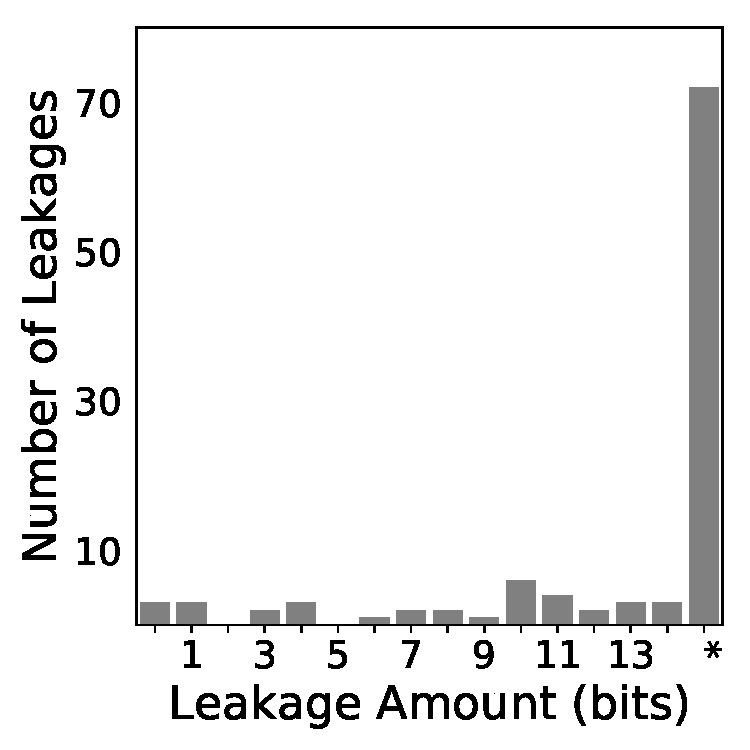
\includegraphics[width=.3\linewidth]{./figures/chapter4/result/RSA-openssl-0-9-7.pdf}
        \label{fig:rsa-1}
    }
    \subfloat[OpenSSL 1.0.2f]{
        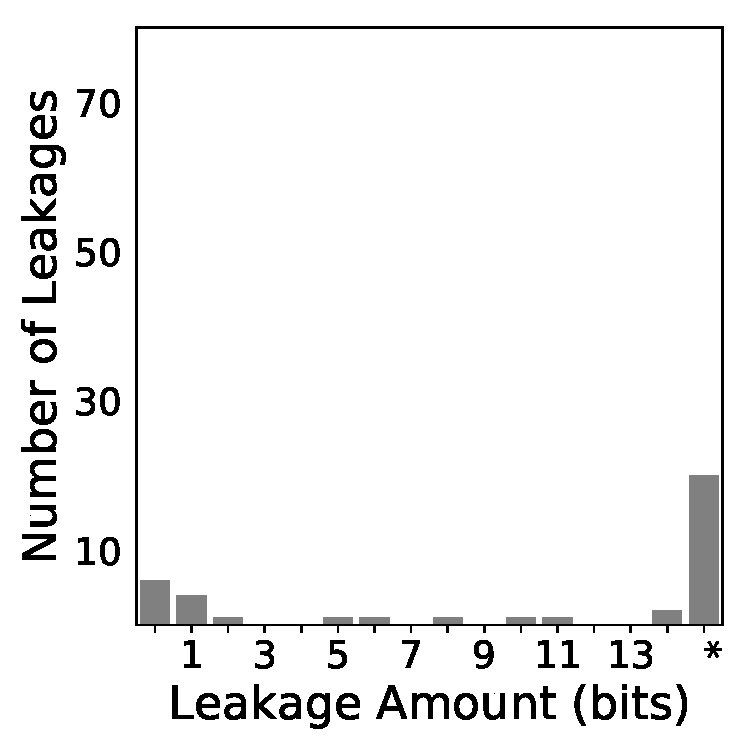
\includegraphics[width=.3\linewidth]{./figures/chapter4/result/RSA-openssl-1-0-2f.pdf}
        \label{fig:rsa-2}
    }
    \subfloat[OpenSSL 1.0.2k]{
        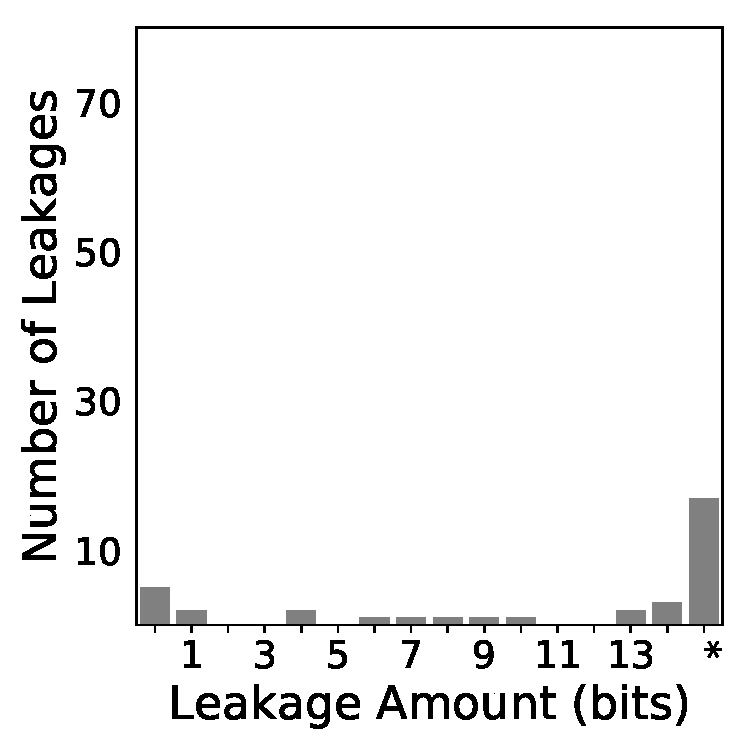
\includegraphics[width=.3\linewidth]{./figures/chapter4/result/RSA-openssl-1-0-2k.pdf}
        \label{fig:rsa-3}
    }
        \hfill

    \subfloat[OpenSSL 1.1.0f]{
        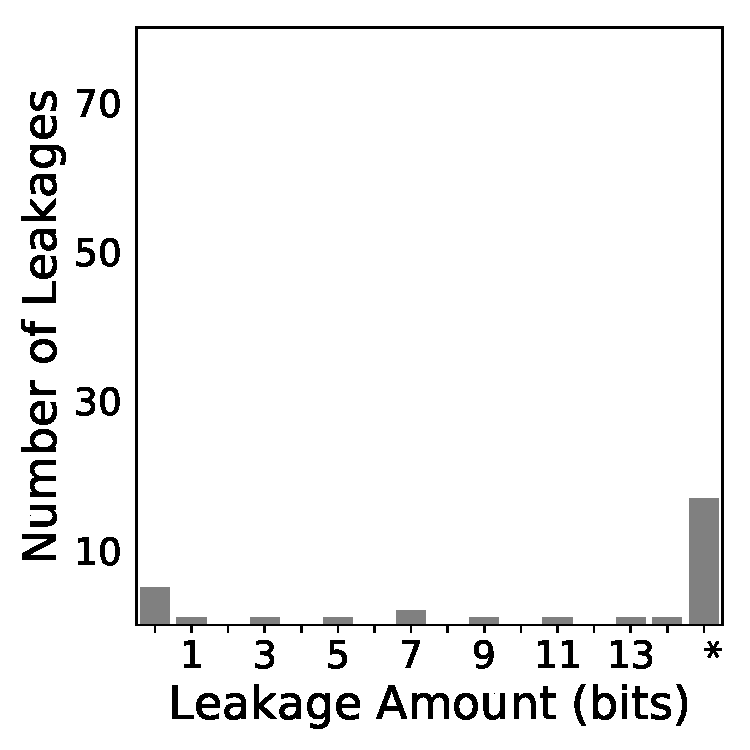
\includegraphics[width=.3\linewidth]{./figures/chapter4/result/RSA-openssl-1-1-0f.pdf}
        \label{fig:rsa-4}
    }
    \subfloat[OpenSSL 1.1.1]{
        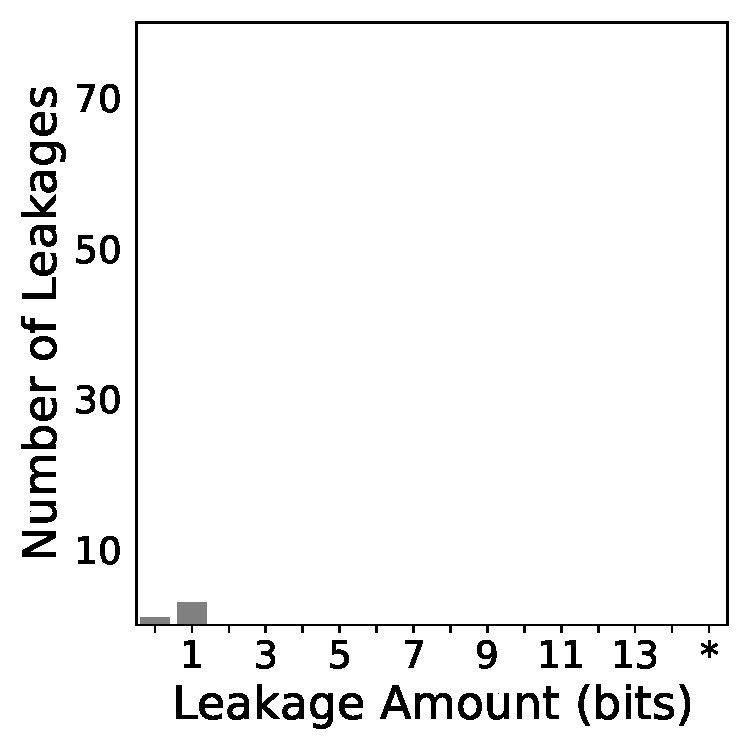
\includegraphics[width=.3\linewidth]{./figures/chapter4/result/RSA-openssl-1-1-1.pdf}
        \label{fig:rsa-5}
    }
    \subfloat[OpenSSL 1.1.1g]{
        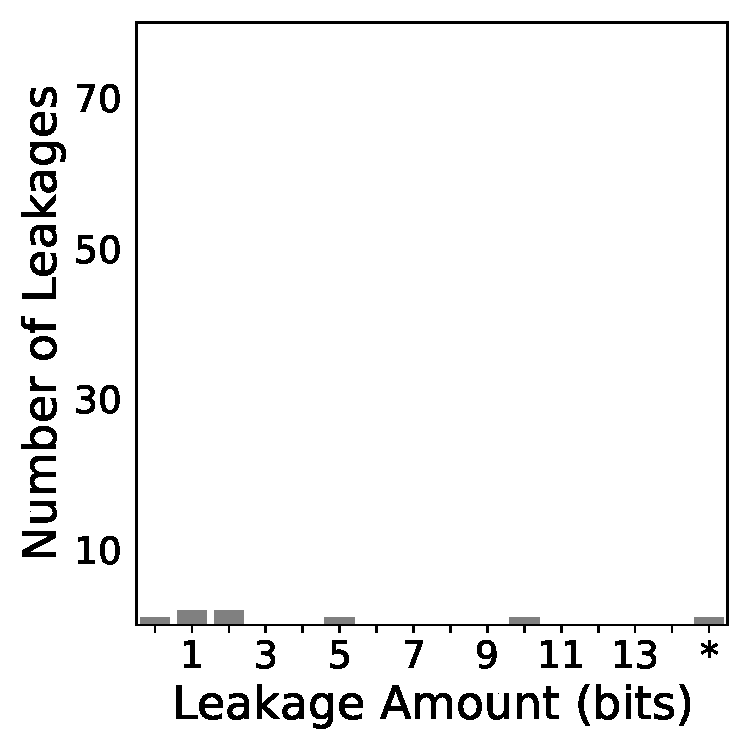
\includegraphics[width=.3\linewidth]{./figures/chapter4/result/RSA-openssl-1-1-1g.pdf}
        \label{fig:rsa-6}
    }
    \caption{Side-channel leakages in different implementations of RSA in OpenSSL\@. 
        We round the number of leaked information into the nearest integer. 
        The mark $*$ means timeout.}
    \label{fig:rsa}
\end{figure*}
We also evaluate \tool{} on RSA.  %, which is available online at the tool release website.
%% \jl{where?}. In general,
%% developers are interested in fixing side-channel vulnerabilities for the RSA implementations.
%% \jl{Then maybe find some space to present these results?}
 As shown in Figure~\ref{fig:rsa}, the result indicates that the newer
versions of OpenSSL leak less information than the earlier
versions. After version 0.9.7g, OpenSSL adopts a fixed-window \textsf{mod\_exp\_mont}
implementation for RSA\@. With this design, the sequence of squares and
multiples and the memory access patterns are independent of the secret key.
\tool{}'s result confirms the new exponentiation implementation has mitigated 
most leakages effectively because the four newer versions have fewer
leakages than version 0.9.7, which introduced this change.
OpenSSL version 1.0.2f, 1.0.2k, and 1.1.0f almost have the
same amount of leakage. We check the ChangeLog and find only one change to
patch vulnerability CVE-2016-0702. 
\tool{} finds OpenSSL 1.1.1 and 1.1.1g have significantly less
leaked information than other versions.
We check the ChangeLog of these two versions and find a claim that
the new RSA implementation adopts ``numerous side-channel attack mitigation'', 
which proves the effectiveness of our quantifying method.
%We also observe the latest version (1.1.1g) contains some new leakages. We have
%contacted the developers and they have confirmed our findings.



Our quantification result shows vulnerabilities
that leak significant amounts of information
are more likely to be fixed in the updated version.
As presented in Figure~\ref{fig:rsa}, 
OpenSSL 0.9.7 has several severe leaks from
function \textsf{bn\_sqr\_comba8}, which is a main 
component of the OpenSSL big number implementation.
Shown in Figure~\ref{fig:old_sqr2}, it has a 
secret-dependent control flow at line 8.
The value of the function parameter \texttt{a} is derived from
the secret key. 
As function \textsf{bn\_sqr\_comba8}
calls the macro (\textsf{sqr\_add\_c2}) multiple times, 
and the code can leak some information each time.
\tool{} indicates the vulnerability is quite severe. 
It was patched in OpenSSL 1.1.1\@. In 
Figure~\ref{fig:new_sqr2}, control-flows transfers are replaced
so there are no leaks in the function
\textsf{sqr\_add\_c2} in OpenSSL 1.1.1\@. We note
that line 4 and 9 in Figure~\ref{fig:old_sqr2} both contain \texttt{if} branches.
However, they are not leaks because
most compilers use \emph{add with carry} instruction to eliminate the branch.
In addition, branches can be compiled into non-branch machine instructions 
with conditional moves. 
We notice a bitwise operation in Libgcrypt 1.8.5 is compiled to a conditional 
jump, which leads to a side-channel leakage.
Therefore, source-level code reviews are not accurate
enough to detect side-channels. 

For vulnerabilities that leak less amount of information,
developers are more reluctant to fix them or fixing them unintentionally. For example, OpenSSL 0.9.7 adds a fixed windows version of function \textsf{BN\_mod\_exp\_mont\_consttime} to replace original function \textsf{BN\_mod\_exp\_mont}.
\tool{} detects a minor vulnerability in the original function that can leak the last bit of the big number \texttt{m}. In the updated version, developers make the fixed windows the default option and rewrite most of the function. However, the leakage site still exists in OpenSSL 1.1.1.
\begin{figure}
    \centering
    \begin{lstlisting}[xleftmargin=.08\textwidth, xrightmargin=.0\textwidth, frame=none]
# define mul_add_c2(a,b,c0,c1,c2)                    \
    t=(BN_ULLONG)a*b;                                \
    tt=(t+t)&BN_MASK;                                \
    if (tt < t) c2++;                                \
    t1=(BN_ULONG)Lw(tt);                             \
    t2=(BN_ULONG)Hw(tt);                             \
    c0=(c0+t1)&BN_MASK2;                             \
    if ((c0 < t1) && (((++t2)&BN_MASK2) == 0)) c2++; \
    c1=(c1+t2)&BN_MASK2; if ((c1) < t2) c2++;
\end{lstlisting}
    \caption{Macro \textsf{sqr\_add\_c2} in OpenSSL 0.9.7}
    \label{fig:old_sqr2}
\end{figure}


\begin{figure}
    \centering
    \begin{lstlisting}[xleftmargin=.08\textwidth, xrightmargin=.0\textwidth, frame=none]
# define mul_add_c2(a,b,c0,c1,c2)      do { \
    BN_ULONG ta = (a), tb = (b);            \
    BN_ULONG lo, hi, tt;                    \
    BN_UMULT_LOHI(lo,hi,ta,tb);             \
    c0 += lo; tt = hi+((c0<lo)?1:0);        \
    c1 += tt; c2 += (c1<tt)?1:0;            \
    c0 += lo; hi += (c0<lo)?1:0;            \
    c1 += hi; c2 += (c1<hi)?1:0;            \
    } while(0)
\end{lstlisting}
\caption{Macro \textsf{sqr\_add\_c2} in OpenSSL 1.1.1}
\label{fig:new_sqr2}
\end{figure}

To evaluate the effectiveness of the leaked bits reported by \tool{}, we conduct a case study of all the leaked sites identified by \tool{} in OpenSSL 1.1.0f. Table~\ref{chapter4:tab:RSAOpenSSL1.1.0} shows the result. First, all leakage sites that leak more than 5 bits information are fixed by developers. Second, for all leakages that are not patched by developers, the quantification result shows that they leak less than 1.0 bits information. The evaluation results show that \tool{} can help developers find severe leakages automatically.

\begin{table}[!ht]
\centering\normalsize
\caption{Leaked Functions in RSA implemented by OpenSSL 1.1.0f. According to \tool{}\cite{bao2021abacus}, the mark ``$*$'' means timeout, which indicates more severe leakages. $0.0$ means very small amount of leakage, but not exactly zero.}\label{chapter4:tab:RSAOpenSSL1.1.0}
\resizebox{\columnwidth}{!}{
\begin{tabular}{lrlrc}
\hline
\textbf{File}  & \textbf{Line Number} & \textbf{Vulnerable Function} & \textbf{Result (bits)} & \textbf{Fixed} \\\hline
bn\_lib.c& 143&BN\_num\_bits\_word&*& \cmark\\
bn\_lib.c& 144&BN\_num\_bits\_word&*& \cmark\\
bn\_lib.c& 145&BN\_num\_bits\_word&17.2 & \cmark\\
bn\_lib.c& 1029&bn\_correct\_top&*&\cmark\\
bn\_lib.c& 639&BN\_ucmp&*&\cmark\\
ct\_b64.c& 164&\_\_udivdi3&5.9 &\cmark\\
bn\_div.c& 330&BN\_div&*&\cmark\\
bn\_gcd.c& 192&int\_bn\_mod\_inverse&1.0 &\xmark\\
bn\_gcd.c& 215&int\_bn\_mod\_inverse&7.9 &\cmark\\
bn\_gcd.c& 237&int\_bn\_mod\_inverse&8.2 &\cmark\\
bn\_gcd.c& 218&int\_bn\_mod\_inverse&14.9 &\cmark\\
bn\_gcd.c& 240&int\_bn\_mod\_inverse&9.2 &\cmark\\
bn\_lib.c& 147&BN\_num\_bits\_word&*&\cmark\\
bn\_lib.c& 152&BN\_num\_bits\_word&12.6 &\cmark\\
bn\_lib.c& 153&BN\_num\_bits\_word&*&\cmark\\
bn\_lib.c& 156&BN\_num\_bits\_word&*&\cmark\\
bn\_div.c& 384&BN\_div&17.2 &\cmark\\
bn\_div.c& 330&BN\_div&11.9 &\cmark\\
bn\_div.c& 334&BN\_div&3.8 &\cmark\\
bn\_exp.c& 622&BN\_mod\_exp\_mont\_consttime&1.0 &\xmark\\
bn\_exp.c& 741&BN\_mod\_exp\_mont\_consttime&1.0 &\xmark\\
bn\_mont.c& 138&BN\_from\_montgomery\_word&*&\cmark\\
bn\_mont.c& 139&BN\_from\_montgomery\_word&*&\cmark\\
bn\_mont.c& 140&BN\_from\_montgomery\_word&*&\cmark\\
bn\_mont.c& 142&BN\_from\_montgomery\_word&*&\cmark\\
bn\_mont.c& 152&BN\_from\_montgomery\_word&*&\cmark\\
bn\_asm.c& 733&bn\_sqr\_comba8&*&\cmark\\
bn\_asm.c& 592&bn\_mul\_comba8&*&\cmark\\
bn\_mont.c& 98&BN\_from\_montgomery\_word&0.0 &\xmark\\
bn\_div.c& 330&BN\_div&0.3 &\xmark\\
bn\_div.c& 330&BN\_div&0.3 &\cmark\\
\hline
\end{tabular}
}
\end{table}




\subsection{Benchmarks}\label{sec:eval_countermeasures}
We also tested \tool{} on a set of small benchmarks.
\subsubsection*{Bit-slicing}
Bit-slicing is an efficient method to construct constant-time implementations to mitigate side-channels. The basic concept is to implement a function in terms of single-bit logical gate operations, such as AND, XOR, OR, and NOT\@.

Since the table look-ups and conditional jumps are replaced with single-bit logical gates, with no secret-dependent memory addresses or control flow, both the data access and control flow types of side-channel leakages are mitigated.
\begin{figure}[h!]
    \centering
    \begin{lstlisting}[xleftmargin=.1\textwidth, xrightmargin=.0\textwidth, frame=none]
uint8_t password = input();

uint8_t SBOX[] = {1, 0, 3, 1, 2, 2, 3, 0};

if (password <= 0b111)      \\Leaks 5 bits of password
    ret = SBOX[password];   \\Leaks 4 bits of password
      \end{lstlisting}
    \caption{SBOX without bitslicing}
    \label{fig:SBOX_da}
\end{figure}


\begin{figure}[h!]
    \centering
    \begin{lstlisting}[xleftmargin=.2\textwidth, xrightmargin=.0\textwidth, frame=none]
uint8_t password = input();
a = *password & 0b001;
b = (*password & 0b010) >> 1;
c = (*password & 0b100) >> 2;
na = ~a & 1;
nb = ~b & 1;
nc = ~c & 1;
t0 = (b & nc);
t1 = (b | nc);
l = (a & nb) | t0;
r = (na & t1) | t0;
ret = l << 1 + r;
\end{lstlisting}
\caption{SBOX with bitslicing}
\label{fig:SBOX_bitslicing}
\end{figure}
We test \tool\ on bit-slicing. We adopt the SBOX
implementations, commonly used in block ciphers such as DES and AES, with and
without bit-slicing, and apply \tool{} to confirm the mitigation. The SBOX implementation with and without bit-slicing are shown in Figure~\ref{fig:SBOX_bitslicing} and Figure~\ref{fig:SBOX_da}, respectively. Considering an SBOX take some bits derived from a password as input and output 2-bit transform result, the plain implementation
has a range check on the password input and a secret-dependent table lookup while bit-slicing does not.

\tool\ reports that there are control-flow and data access types of leakages
in the non-bit-slicing implementation (line 6 and line 7 in Figure~\ref{fig:SBOX_da}). The number of leaked bits is
5.0 and 4.4, respectively. At line 6, according to Definition~\ref{chapter4:def}, the
input set $K$ is $[0,2^8-1]$, the observed input set $K^o$ is $[0,2^3-1]$. Thus,
the leakage $L_{\beta(k)\rightarrow o}$ based on the observation ($o$) is
$L_{\beta(k)\rightarrow o} = \log_2{|K|} - \log_2{|K^o|} = 8-3 = 5$ bit, which
confirms the result from \tool. Similarly, we can verify the result of other
leakage sites. \tool{} reports no leakage on the bit-slicing implementation.


\subsubsection*{Lookup Table}
\begin{figure}[h]
\centering
    \begin{lstlisting}[xleftmargin=.05\textwidth, xrightmargin=.05\textwidth, frame=none]
static const uint8_t T[1024] = {
      0x63U, 0x7cU, 0x77U, 0x7bU, 0xf2U, 0x6bU, 0x6fU, 0xc5U,
      0x30U, 0x01U, 0x67U, 0x2bU, 0xfeU, 0xd7U, 0xabU, 0x76U,
...
output = (T[(key[0]>>24)] << 24) ^
         (T[(key[1]>>16) & 0xff] << 16) ^
         (T[(key[2]>>8) & 0xff] << 8) ^
         (T[(key[3]) & 0xff]);
\end{lstlisting}
  \caption{Lookup tables with small entries.}\label{fig:chapter4:small_lookup}
\end{figure}

\begin{figure}[h]
\centering
    \begin{lstlisting}[xleftmargin=.05\textwidth, xrightmargin=.05\textwidth, frame=none]
static const uint32_t T[256] = {
    0xc66363a5U, 0xf87c7c84U, 0xee777799U, 0xf67b7b8dU,
    0xfff2f20dU, 0xd66b6bbdU, 0xde6f6fb1U, 0x91c5c554U,
    0x60303050U, 0x02010103U, 0xce6767a9U, 0x562b2b7dU,
    0xe7fefe19U, 0xb5d7d762U, 0x4dababe6U, 0xec76769aU};
...
output = (T[(key[0]>>24)] << 24) ^
         (T[(key[1]>>16) & 0xff] << 16) ^
         (T[(key[2]>>8) & 0xff] << 8) ^
         (T[(key[3]) & 0xff]);
\end{lstlisting}
  \caption{Lookup tables with big entries.}\label{fig:chapter4:big_lookup}
\end{figure}


Considering the cache-collision timing attack~\cite{Bonneau11894063_16}, the
probability of leakage decreases when the lookup table entry or element size gets
smaller. We analyze the table lookup with \tool{}. It is a common operation used by symmetric ciphers such as AES. Figure~\ref{fig:chapter4:big_lookup} is from the original AES reference implementation. It uses a lookup table and each entry is 4 bytes, which is vulnerable to side-channel attacks. Most cryptography libraries adopted the mitigated version, shown in Figure~\ref{fig:chapter4:small_lookup}. \tool{} reports three leakage sites for
each lookup table, with 4.0 bits for the table with smaller entries and 2.0
bits for the table with bigger entries, confirming the theory.
The evaluation result shows the version with smaller lookup tables leaks less information, which confirm the effectiveness of the mitigation technique. 



\subsubsection*{Password Checker}

\begin{figure}[h]
    \begin{lstlisting}[xleftmargin=.2\textwidth, xrightmargin=.0\textwidth, frame=none]
bool pwcheck(uint8_t *key, uint8_t *pub) {
  for (int i = 0; i < 2; ++i) {
    if (key[i] != pub[i]) {
      return false;
    }
  }
  return true;
}
\end{lstlisting}\caption{A vulnerable password checker.}\label{fig:chapter4:pwcheck1}
\end{figure}

\begin{figure}[h]
    \begin{lstlisting}[xleftmargin=.2\textwidth, xrightmargin=.00\textwidth, frame=none]
bool pwcheck(uint8_t *key, uint8_t *pub) {
  bool matched = true;
  for (int i = 0; i < 2; ++i) {
    if (pub[i] != key[i]) 
      matched = false;
  }
  return matched;
}
\end{lstlisting}\caption{A safe password checker.}\label{fig:chapter4:pwcheck2}
\end{figure}

We illustrate the quantification method on two password checking examples.  As shown in Figure~\ref{fig:chapter4:pwcheck1}, the version is vulnerable to side-channel attacks because of the early return at line 4. If the first bytes of \textsf{key} and \textsf{pub} are the same, the function will continue running and access the second byte. Figure~\ref{fig:chapter4:pwcheck2} fixes the vulnerability because the function will continue comparing the second byte even if the first byte is different.  \tool{} identifies the leakage site in Figure~\ref{fig:chapter4:pwcheck1} successfully, and estimates the amount of leakage is $16$ bits. 


